% @author Tobias Wulf
% thesis root document

\documentclass[
  a4paper,            % DIN A4
  DIV=10,             % Schriftgröße und Satzspiegel
  oneside,            % einseitiger Druck
  BCOR=5mm,           % Bindungskorrektur
  parskip=half,       % Halber Abstand zwischen Absätzen
  numbers=noenddot,   % Kein Punkt hinter Kapitelnummern
  bibtotoc,           % Literaturverzeichnis im Inhaltsverzeichnis
  listof=totoc        % Abbildungs- und Tabellenverzeichnis im Inhaltsverzeichnis
]{scrreprt}
\usepackage{./style/thesisstyle}
  
\makeglossaries           % create all glossary entries (remember: run makeglossaries manually)
\makeindex
\loadglsentries[main]{./glossaries/glossary}  % load acronym, symbol and glossarie entries
\loadglsentries[\acronymtype]{./glossaries/acronyms}
\loadglsentries[symbols]{./glossaries/symbols}

\addbibresource{./literature/literature.bib}

\sisetup{locale = DE}     % siunitx locale setup
%\DeclareSIUnit \fps{fps}  % a custom unit (usage: \SI{24}{\fps})

\begin{document}
% !TEX root = ../thesis.tex
%
% configurations
%

% text field
%-> replace supervisor names with correct ones
\firstSupervisor{Prof. Dr. Karl-Ragmar Riemschneider}
\secondSupervisor{Prof. Dr. Klaus Jünemann}

% text field
%-> replace title with your thesis title
\thesisTitle{Winkelmessung durch magnetische Sensor-Arrays und Toleranzkompensation mittels Gauß-Prozess}
\thesisTitleEN{Angular Measurement by Magnetic Sensor Arrays and Tolerance Compensation by Gaussian Process}

% text field
%-> replace the key words with your own key words
\keywordsDE{Sensor-Array Simulation, Dipol, Magnetfeld, Kugelmagnetapproximation, TMR, TDK TAS2141, AMR, NXP KMZ60, Toleranzkompensation, Gauß'sche Prozesse, Kovarianz, Kovarianzmatrix, Regression, Winkelvorhersage, Logarithmische Modellplausibilität, Standardisierter Logarithmischer Modellverlust, Minimierungsproblem, Optimierung, ASIC-Modell}

\keywordsEN{Sensor Array Simulation, Dipole, Magnetic Field, Sperical Magnet Approximation, TMR, TDK TAS2141, AMR, NXP KMZ60, Tolerance Compensation, Gaussian Processes, Covariance Covariance Matrix, Regression, Angular Prediction, Logarithmic Marginal Likelihood, Standardized Logarithmic Loss, Minimization, Optimization, ASIC Model}

% text field
%-> replace the text with a description of the thesis
\abstractDE{Die vorliegende Bacheloarbeit umfasst den Aufbau und die Verbesserung von Simulationssoftware und Modellen für die physikalische Simulation eines tunnel-magnetoresistiven Sensor-Arrays sowie die mathematische Simulation eines dazugehörigen auswertenden  ASIC-Modells. Das mathematische ASIC-Modell für die Auswertung der Sensor-Array-Simulationsdaten beruht auf einem Regressionsverfahren für Gauß'sche Prozesse. In Vorarbeiten sind Grundlagen zur physikalischen und mathematischen Simulation der Modelle geschaffen worden, die im Rahmen dieser Arbeit zu einer modular aufgebauten Software zusammengeführt werden. Des Weiteren wird das mathematische ASIC-Modell in Bezug auf Modellressourcen und maschinelle Lernfähigkeit weiterführend optimiert und verbessert sowie durch Algorithmen zur Modelloptimierung ergänzt. Abschließend werden in dieser Arbeit Experimente zur Funktionalität, Modelloptimierung und Fähigkeit zur Toleranzkompensation des Gesamtsystems durchgeführt.}

\abstractEN{This bachelor thesis covers the construction and improvement of simulation software and models for the physical simulation of a tunnel magnetoresistive Sensor Array as well as the mathematical simulation of an associated evaluating ASIC model. The mathematical ASIC model for the evaluation of the Sensor Srray simulation data is based on a regression method for Gaussian Processes. In preliminary work, basic principles for the physical and mathematical simulation of the models have been created, which will be combined into a modular software within the scope of this work. Furthermore, the mathematical ASIC model will be further optimized and improved with respect to model resources and machine learning capability, and supplemented by algorithms for model optimization. Finally, experiments on the functionality, model optimization and tolerance compensation capability of the overall system are carried out in this thesis.}

% text field
%-> replace jon with your name
\thesisAuthor{Tobias Wulf}

% text field
%-> enter the submission date
\submissionDate{08. Juni 2021}

% switch - uncomment only one
%-> uncomment NDA or public
%\NDA{yes}
\NDA{no}

% switch - uncomment only one
%-> uncomment cover or cover Corporate Design 2017
%\Cover{CD2017}
%\Cover{CD2017NoLogo}
\Cover{Std2018}

% switch - uncomment only one
%-> uncomment to show list of figures or not
\ListOfFigures{yes}
%\ListOfFigures{no}

% switch - uncomment only one
%-> uncomment to show list of tables or not
\ListOfTables{yes}
%\ListOfTables{no}

% switch - uncomment only one
%-> uncomment to show list of accronyms or not
\ListOfAccronyms{yes}
%\ListOfAccronyms{no}

% switch - uncomment only one
%-> uncomment to show list of symbols or not
\ListOfSymbols{yes}
%\ListOfSymbols{no}

% switch - uncomment only one
%-> uncomment to show list of glossary entries or not
\Glossary{yes}
%\Glossary{no}

% switch - uncomment only one
%-> uncomment the study course you are in
%\studycourse{ITS}
%\studycourse{TI}
%\studycourse{AI}
%\studycourse{WI}
\studycourse{EI}
%\studycourse{REE}
%\studycourse{BMT}
%\studycourse{MAI}
%\studycourse{MIK}
%\studycourse{MA}
    % load all settings

\hyphenation{Ba-che-lor-the-sis Mas-ter-the-sis}

% Cover page here, no page number
\ICoverPage

% PDF Metadata
\input{./style/metadata}

% Titlepage is page one even if the number is not shown.
\pagenumbering{roman}
% Title page here
\input{./style/titlepage}

% Abstract page here
% !TEX root = ../thesis.tex
%
% abstract page
% @author Thomas Lehmann
%
\newpage
\thispagestyle{plain}
\clearpage
\hfuzz=12pt       % suppress warnings due to extenstion onto page margins

\textbf{\IthesisAuthor}

\vspace{0.3cm}
\textbf{Thema der Arbeit}

\IthesisTitle

\vspace{0.3cm}
\textbf{Stichworte}

\IkeyWordsDE

\vspace{0.3cm}
\textbf{Kurzzusammenfassung}

\begin{minipage}{\textwidth}
\IabstractDE
\end{minipage}

%\vspace{1.0cm}
\clearpage
\textbf{\IthesisAuthor}

\vspace{0.3cm}
\textbf{Title of Thesis}

\IthesisTitleEN

\vspace{0.3cm}
\textbf{Keywords}

\begin{minipage}{\textwidth}
\IkeyWordsEN
\end{minipage}

\vspace{0.3cm}
\textbf{Abstract}

\IabstractEN

\newpage
\thispagestyle{plain}
\clearpage
\hfuzz=12pt       % suppress warnings due to extenstion onto page margins

\chapter*{Danksagung}

\begin{minipage}{\textwidth}
Ich möchte mich bedanken, dass mir die Möglichkeit gegeben worden ist, im Rahmen des Forschungsprojektes ISAR, meine Bachelorarbeit zu schreiben. Meinen herzlichen Dank gilt dabei Herr Prof. Dr.-Ing. Karl-Ragmar Riemschneider als mein betreuender Erstprüfer. Herr Prof. Dr.-Ing. Riemschneider ermöglichte mir die Mitarbeit am Forschungsprojekt zu einem Zeitpunkt, als durch wirtschaftliche Restrukturierungen seitens meines Arbeitgebers, die eigentlich vereinbarte Bachelorarbeit wegbrach und mein Abschluss dadurch gefährdet wurde. Das möchte ich an dieser Stelle besonders hervorheben. Ebenso möchte ich meinen Dank an Herr Prof. Dr. Klaus Jünemann als Zweitprüfer meiner Bachelorarbeit aussprechen.
\newline


Des Weiteren möchte ich mich bei Herr M.Sc. Thorben Schüthe und Herr Dipl.-Ing. Günter Müller bedanken, die mir während der gesamten Bearbeitungszeit mit fachlichen Rat geholfen haben. Natürlich gilt mein Dank auch der gesamten Arbeitsgruppe Sensorik, in deren Mitte ich offenherzig aufgenommen wurde und die mir eine angenehme und anregende Arbeitsatmosphäre bat.
\newline


Ich möchte an dieser Stelle ebenfalls meinen beruflichen Wegbegleitern und Förderern Herr Dipl.-Ing. Markus Piorek, Herr Dipl.-Ing. Alexander Geist und Herr Dr.-Ing. Martin Krey meinen Dank bekunden. Für all den Zuspruch und Offenheit, die mir während meines nebenberuflichen Studiums entgegengebracht worden sind.
\newline


Ganz besonderen Dank möchte ich meiner Familie und meiner Freundin schenken. Ihr habt an mich geglaubt und seit mit mir zusammen durch alle Höhen und Tiefen gegangen. Euer Verständnis und Vertrauen haben mich stets beflügelt.
\newline


Vielen Dank!
\end{minipage}

% Table of contents here
\tableofcontents

% Uncomment if list of source code is needed (rarely).
%\lstlistoflistings  % requires package listings, needs to uncommenting of usepackage

% path to the chapters folder is set to find the images used there
\graphicspath{ {./chapters/} {.chapters/images}}

% Chapters
\clearpage
\pagenumbering{arabic}
% Add additional chapters here
% !TEX root = ../thesis.tex
% introduction
% @author Tobias Wulf
%

\chapter{Motivation 0.0.1 17.02.2021}

Neuentwicklungen in der Halbleitertechnik, auf Basis des \gls{gl:tmr}s, ermöglichen den Aufbau komplexerer Sensorstrukturen \cite{Schuethe2019}. Die \gls{gl:ags} an der \gls{gl:haw} erforscht moderne Ansätze der Signalverarbeitung für neugewonnene Sensorstrukturen, verwirklicht als magnetische Sensor-Arrays. Durch den Aufbau von Sensoren als Arrays, bieten sich Möglichkeiten zur Nutzung von Algorithmen und Regressionsverfahren an, die eine Kompensation und Detektion von mechanische Toleranzen zulassen \cite{Schuethe2020}.
\newline
Das Verarbeiten einer Vielzahl an Messwerten, bedingt durch Sensor-Array-Strukturen, ist hierbei eine der Herausforderungen die es zu bewältigen gilt. Mit Hilfe moderner Algorithmen, die Ansätze des maschinellen Lernens beinhalten, ergeben sich weitere Problemstellungen in Bezug auf Modellabbildung- und Optimierung.
Das übergeordnete Ziel bei der Lösung und Bewältigungen der einzelnen Etappen ist die Verbesserung der Messgenauigkeit, indem individuelle Abweichungen des Sensors einem geeigneten Modell antrainiert und Modellparameter optimiert werden. Moderne Regressionsverfahren liefern dabei statistische Ansätze um geeignete Qualitätskriterien zu bilden und somit trainierte Modelle und ihre Messwertgenauigkeit zu bewerten.

\input{chapters/1-1-Zielstellung}
% !TEX root = ../thesis.tex
% basics
% @author Tobias Wulf
%

\chapter{Grundlagen 0.0.2 19.02.2021}\label{ch:grundlagen}

Das Fundament für die Drehwinkelerfassung mittels magnetischen Sensor-Array und lernender Signalverarbeitung 
\cite{Schuethe2019}\cite{Schuethe2020a}\cite{Schuethe2020}, die auf Regressionsverfahren für Gauß-Prozesse 
\cite{Rasmussen2006} aufbauen, bildet sich durch Abstandmessungen von Winkelpositionen auf einer Kreisbahn. Für eine
anschauliche Erklärung der Zusammenhänge soll als Einstieg in die Grundlagen, das Prinzip anhand eindimensionaler 
Vektorfelder zweier Winkelstellungen $A$ und $B$ gezeigt werden. Das entspräche einem Anwendungsfall einfacher und 
heute erhältlicher magnetischer Sensoren, wie dem KMZ60 \cite{NXPSemiconductors2014} von NXP, oder dem  TAS2141-AAAB 
\cite{TDK2016} der Firma TDK. Die Verfahrensgrundlage, der eindimensionalen Betrachtung, wird in der Verwendung von 
Sensor-Arrays adaptiert und durch geeignete Rechen- und Normierungsverfahren auf die Problemstellung eines 
höherdimensionalen Systems projiziert.


Der in \autoref{fig:veranschaulichung-sensor-ic} gezeigte Anwendungsfall, soll hier als Grundlage der Erläuterungen 
dienen. Genaue technische und physikalische Größenzusammenhänge sind vorerst vernachlässigt. 
\autoref{fig:veranschaulichung-sensor-ic} zeigt eine kreisförmige Rotation des Gebermagneten um seine $Z$-Achse. 
Entsprechend rotiert das Magnetfeld bei Drehung des Magneten mit. Der darunter liegende Sensor erfasst die 
Magnetfeldstärke $\vec{H}$ des Gebermagnetfeldes. Die Winkelstellung $\alpha$ des Magneten kann dabei nicht direkt 
erfasst werden. Der Sensor misst, die zueinander und zur Rotationsachse orthogonal stehenden, $X$- und $Y$-Komponenten 
der Gebermagnetfeldstärke $\vec{H}$ und setzt diese in elektrische Spannungssignale um. Bedingt durch die Kreisbewegung 
und Orthogonalität, lässt sich die Winkelstellung mittels einfacher Vektorrechnung bestimmen. 


\clearpage


Bei idealer und gleichbleibender Position des Magneten in Relation zum Sensor, beschreiben die aufgenommen Messpunkte 
eine Kreisbahn mit konstanten Bahnradius $r$ und Winkelstellung $\alpha$ des Gebermagneten. 
\autoref{fig:kreisdarstellungwinkelabstand} zeigt den Zusammenhang für zwei erfasste Winkelstellungen $A$ und $B$. Es 
ergeben sich für die beiden Winkelstellungen $A\mapsto\alpha_1$ und $B\mapsto\alpha_2$ folgende vektorielle 
Zusammenhänge in \autoref{eq:vektorenab}.


\begin{equation}\label{eq:vektorenab}
\begin{aligned}
	A &= 
		\begin{pmatrix} 
			a_x \\
			a_y 
		\end{pmatrix}
	  &= 
		\begin{pmatrix} 
			r \cdot \cos(\alpha_1) \\
			r \cdot \sin(\alpha_1) 
		\end{pmatrix} \\
	B &=
		\begin{pmatrix} 
			b_x \\
			b_y 
		\end{pmatrix}
	  &= 
		\begin{pmatrix} 
			r \cdot \cos(\alpha_2) \\
			r \cdot \sin(\alpha_2) 
		\end{pmatrix} \\
\end{aligned}
\end{equation}


Die vom Sensor erfassten und umgewandelten $X$- und $Y$-Komponenten der Messpunkte $A$ oder $B$, bilden 
eindimensionale Vektorfelder. Über ihren Betrag lässt sich der Bahnradius $r$ ermitteln, zu sehen in 
\autoref{eq:vektor2norm}. Allgemein ist der Betrag eines Vektors über die Vektor-2-Norm zu berechnen. Diese Norm 
wird oft auch als euklidische Norm bezeichnet.


\begin{equation}\label{eq:vektor2norm}
	\begin{aligned}
	r &:= &\|A\|_2 &= &\sqrt{\sum_{i=1}^{n}|A_i|^2} &= &\sqrt{|a_x|^2 + |a_y|^2} &= &|A| &= &konst. \\
	  &&&&&\equiv \\
	  &   &\|B\|_2 &= &\sqrt{\sum_{i=1}^{n}|B_i|^2} &= &\sqrt{|b_x|^2 + |b_y|^2} &= &|B| &= &konst.
	\end{aligned}
\end{equation}


Der direkte Winkelabstand zwischen $A$ und $B$ kann geometrisch, wie in \autoref{fig:kreisdarstellungwinkelabstand} 
gezeigt, über die Abstandsquadrate der vektoriellen Anteile ermittelt werden und ist gleich der Kantenlänge des 
Quadrates zwischen den Punkten $A$ und $B$. Entsprechend der Kreisbahnnormierung für die Messpunkte, ist diese Form der 
Abstandsermittlung als euklidischer Abstand $d_E\langle A,B \rangle$ bezeichnet. Zu berechnen ist der Abstand 
$d_E\langle A,B \rangle$ nach \autoref{eq:euklidischerabstand} als Vektor-2-Norm der vektoriellen Differenz von $A$ und 
$B$.


\begin{equation}\label{eq:euklidischerabstand}
	d_E\langle A,B \rangle = \|A - B\|_2 = \sqrt{\sum_{i=1}^{n}(A_i - B_i)^2} = \sqrt{(a_x - b_x)^2 + (a_y - b_y)^2}
\end{equation}


\clearpage


Für den euklidischen Abstand zwischen zwei Winkelstellungen $d_E\langle A,B \rangle$ und das Quadrat des Abstandes 
$d_E^2\langle A,B \rangle$ muss die Dreiecksungleichung nach \autoref{eq:v2ndreiecksungleichung} für allgemeine 
Vektor-2-Normen gelten \cite{vandeGeijn2014}. Dieser Zusammenhang kann genutzt werden um eine Kreisbahn zu 
approximieren, wenn der Bahnradius $r$ nicht konstant und $\|A\|_2 \ne \|B\|_2$ ist. 


\begin{equation}\label{eq:v2ndreiecksungleichung}
	\begin{gathered}
	\big|\|A\|_2 - \|B\|_2\big| \le \|A \pm B\|_2 \le \big|\|A\|_2 + \|B\|_2\big| \\
	\Downarrow \\
	\big(\|A\|_2 - \|B\|_2\big)^2 \le \|A - B\|_2^2 = d_E^2\langle A,B \rangle
	\end{gathered}
\end{equation}


\begin{figure}[tbph]
	\centering
	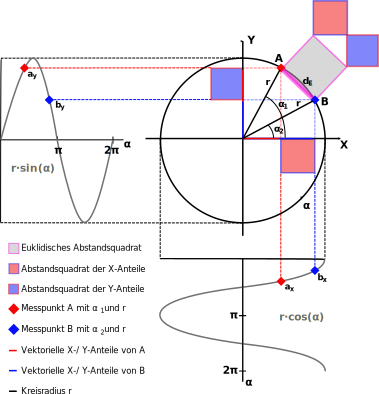
\includegraphics[width=0.7\linewidth]{chapters/images/Kreisdarstellung_Winkelabstand}
	\caption[Allg. Kreisdarstellung des euklidischen Winkelabstands]{Allg. Kreisdarstellung des euklidischen 
	Winkelabstands. Die Kreisdarstellung zeigt den euklidischen Winkelabstand zweier Winkelmesspunkte $A$ und $B$ 
	mit gleichen Kreisradius $r$. Der euklidische Abstand, bzw. das Abstandsquadrat, zwischen den Winkelposition 
	$A$ und	$B$ ist zerlegt in Abstandsquadratanteile. Die Abstandquadratanteile ergeben sich aus der vektoriellen 
	Zusammensetzung in $X$-/ $Y$-Anteile für die einzelnen Messpunkte $A$ und $B$.}
	\label{fig:kreisdarstellungwinkelabstand}
\end{figure}


\clearpage


Bei konstant bleibenden Bahnradius $r$ befindet sich der Abstand $d_E\langle A,B \rangle$ im Intervall $0 \le 
d_E\langle A,B \rangle \le \sqrt{2}\cdot r$. Die Winkelstellungen des Gebermagnet lassen sich über die Vektoranteile 
der Messpunkte und den Bahnradius $r$ berechnen. Also eine Überführung aus kartesischer Darstellung der Messpunkte in 
ihre Polarkoordinaten aus \autoref{eq:vektorenab}. Hier in \autoref{eq:umrechnungpolar} für beliebige Messpunkte auf 
der Kreisbahn gezeigt.

\begin{equation}\label{eq:umrechnungpolar}
	\cos(\alpha) = \frac{x}{r} \quad\sin(\alpha) = \frac{y}{r} \quad\tan(\alpha) = \frac{y}{x}
\end{equation}

\begin{equation}
	\alpha' = 
	\begin{cases}
		+\arccos\left(\frac{x}{r}\right)        & \quad\text{f. } \arcsin\left(\frac{y}{r}\right) \ge 0\\
		-\arccos\left(\frac{x}{r}\right) + 2\pi & \quad\text{f. } \arcsin\left(\frac{y}{r}\right) < 0
	\end{cases}
\end{equation}


\begin{figure}[tbph]
	\centering
	\includegraphics[width=0.5\linewidth]{chapters/images/Winkelumrechnung_Polar}
	\caption[Winkelrückrechnung mit Bereichsumschaltung]{Winkelberechnung mit Bereichsumschaltung. Die Berechnung des 
	Winkel $\alpha'$ erfolgt über die $\arccos$ und $\arcsin$ Funktion, bzw. die vektoriellen Anteile der Messpunkte. 
	Die $\arcsin$ Funktion bildet dabei den Schwellwert für die Bereichsumschaltung um eine volle Rotation abzubilden.}
	\label{fig:winkelumrechnungpolar}
\end{figure}



\begin{itemize}
	\item Einleitung Aufgabenfeld
	\item Einheitskreis
	\item Bezug zur Drehwinkelerfassung und Sensorapplikation
\end{itemize}
\clearpage


\section{Magnetische Sensorentypen und mechatronische Anwendung}\label{sec:magnetische-sensorentypen}
	\begin{itemize}
		\item Die Technologie mit der ein Sensorkopf realisiert ist, klassifiziert in der Regel die Sensorbezeichnung. Anhänge in der Bezeichnung wie AMR oder TMR, geben somit Auskunft darüber welche Technologie für die Realisierung des Sensorkopfes die Grundlage bildet.
		\item Anwendungsfall Winkelmessung
		\item Aufbau Sensorbrücke TMR (Umriss aus Datenblatt)
		\item Ausblick TMR Drehzahlmessung und Strommessung
	\end{itemize}

Die Konzipierung magnetischer Sensoren für die Drehwinkelerfassung richtet sich auf die Erfassung eines kreisförmigen 
Anregungsmagnetfeldes mit einer Feldstärke $\vec{H}$. Also ein kreisförmig rotierendes Magnetfeld, zumeist erzeugt 
durch einfache zweipolige Gebermagneten. Die räumliche Anordnung der Anwendung ist in 
\autoref{fig:veranschaulichung-sensor-ic} zu sehen. Das Magnetfeld rotiert um die $Z$-Achse des Sensors. Zur Detektion 
des Magnetfeldes bzw. seiner Rotation sind dessen Anteile in $X$- und $Y$-Richtung genutzt. Die Nord-Südausrichtung des 
Gebermagneten liegt dabei in der $X$- bzw. $Y$-Achse der Anwendung, bestehend aus Magnet und Sensor. Die Magnetfeldst 
des Gebermagneten ist durch seine vektoriellen Anteile in $X$, $Y$ und $Z$-Richtung beschrieben \cite{Pape2017}. Weitere

\begin{equation}\label{eq:hfeldanteile}
\vec{H} = \begin{pmatrix}H_x\\H_y\\H_z\end{pmatrix}
\end{equation}

Die Einheit der Feldstärke $\vec{H}$ ist $\SI{}{\ampere\per\metre}$. Gängige Feldstärkengrößen für eine magnetische 
Anregung von Drehwinkelsensoren liegen Bereich $\SI{}{\kilo\ampere\per\metre}$.

\begin{figure}[tbph]
	\centering
	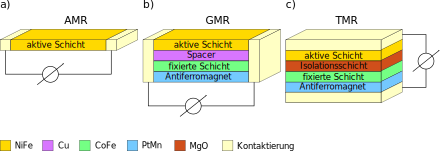
\includegraphics[width=\linewidth]{chapters/images/MR_Schichtmodelle}
	\caption[Schichtmodelle dreier magnetoresistive Effekte]{Schichtmodelle dreier magnetoresistive Effekte. a) 
	\gls{gl:amr}, schwache Widerstandsänderung. b) \gls{gl:gmr} stärkere Widerstandsänderung. c) \gls{gl:tmr} stärkste 
	Widerstandsänderung. Grafik entnommen aus \cite{Lemme2016}.}
	\label{fig:mrschichtmodelle}
\end{figure}



\begin{figure}[tbph]
	\centering
	\includegraphics[width=\linewidth]{chapters/images/TMR_Drehwinkelapplikation}
	\caption[TMR Drehwinkelapplikation]{TMR Drehwinkelapplikation. Schematisch gezeigt für eine volle Rotation des 
	Gebermagneten um $\SI{360}{\degree}$. Zu sehen sind die um $\SI{90}{\degree}$ verdrehten Wheatstone-Brücken des 
	Sensors. Die Brücken bilden, bei rotierenden Gebermagnetfeld, eine Sinus- und Cosinus-Funktion nach. Die Pfeile in 
	den einzelnen Widerständen weisen auf ihre magnetische Ausrichtung hin. Grafik entnommen und bearbeitet aus 
	\cite{Schuethe2020a}.}
	\label{fig:tmrdrehwinkelapplikation}
\end{figure}


\clearpage


\section{Kennfeldmethode zur Charakterisierung von Sensoren}\label{sec:kennfeldmethode-zur-charakterisierung}
	\begin{itemize}
		\item Überleitung von Sensorbrückenschaltung
		\item Messprinzip für das Erstellen der Sensorbrücken-Kennfelder
		\item Festlegung von Arbeitsbereich (Plateau TMR), Sättigung (KMZ60)
		\item Dimensionierung des Stimulus, Dipole Anregung
	\end{itemize}
	
	
	\clearpage
	\begin{figure}[tbph]
		\centering
		\includegraphics[width=\linewidth]{chapters/images/Magnetfeldstimulus_Kennfeldmethode}
		\caption[Magnetfeldstimulus zur Erzeugung von Sensorkennfeldern]{Magnetfeldstimulus zur Erzeugung von 
		Sensorkennfeldern. Es sind die Bestandteile des magnetischen Sensorstimuli dargestellt, die zum Ausmessen des 
		Sensorkennfeldes in $H_x$- und $H_y$-Richtung verwendet worden sind. Es ist das Prinzip des Verfahrens 
		dargestellt. In a) und b) ist die Dreiecksmodulation des magnetischen Anregungsfeldes abgebildet. Für a) die 
		$H_x$-Feldanregung mit Cosinus-Trägerwelle und für b) die $H_y$-Feldanregung mit Sinus-Trägerwelle. Es sind für 
		beide Anregungsrichtungen niedrige Frequenzen gewählt um ein quasi-statisches Anregungsmagnetfeld zu erzeugen. 
		Es ergeben sich für die Betragsamplitude des Stimulus, in polarer Darstellung c) und d), konzentrische 
		Trajektorien. Diese verlaufen von Innen nach Außen für die steigende Flanke der Amplitudenmodulation c) und von 
		Außen nach Innen für die fallende Flanke d). Die Dreieckmodulationsfrequenz liegt bei $f_m = \SI{0.1}{\hertz}$ 
		und einer Trägerwellenfrequenz $f_c = \SI{3.2}{\hertz}$. Grafik nachempfunden aus \cite{Schuethe2019}.}
		\label{fig:magnetfeldstimuluskennfeldmethode}
	\end{figure}
	
	
	\clearpage
	\begin{figure}
		\centering
		\includegraphics[width=\linewidth]{chapters/images/TDK_Kennfelder}
		\caption[TDK TAS2141-AAAB Winkelsensorbrückenkennfelder]{TDK TAS2141-AAAB Winkelsensorbrückenkennfelder. Zu 
		sehen sind die Kennfelder der Cosinus-Brücke a) und b). Darunter befinden sich die Kennfelder der Sinus-Brücke 
		c) und d). Die Kennfelder für beide Brücken a) und c) beziehen sich auf die steigenden Flanke der 
		Amplitudenmodulation aus \autoref{fig:magnetfeldstimuluskennfeldmethode} und die in b) bzw. d) gezeigten 
		Kennfelder sind gewonnen aus der fallenden Flanke. Die Brückenkennfelder sind normiert in 
		$\SI{}{\milli\volt\per\volt}$. Für eine Spannungsausgabe in Betriebsspannungsniveau ist keine zusätzliche 
		Verstärkung notwendig. Die Kennfelder besitzen, jeweils in $H_x$- und $H_y$-Richtung, eine Schrittweite von 
		$\SI{0.1961}{\kilo\ampere\per\metre}$ und sind skaliert von $\SI{-25}{\kilo\ampere\per\metre}$ bis 
		$\SI{+25}{\kilo\ampere\per\metre}$. Somit ergibt sich eine Bildauflösung für ein Kennfeld von $256 \times 256$ 
		Messpunkten. Grafik nachempfunden aus \cite{Schuethe2019}.}
		\label{fig:tdkkennfelder}
	\end{figure}
	
	
	\clearpage
	\begin{figure}[tbph]
		\centering
		\includegraphics[width=\linewidth]{chapters/images/KMZ60_Kennfelder}
		\caption[NXP KMZ60 Winkelsensorbrückenkennfelder]{NXP KMZ60 Winkelsensorbrückenkennfelder. Zu sehen sind die 
		Kennfelder der Cosinus-Brücke a) und b). Darunter befinden sich die Kennfelder der Sinus-Brücke c) und d). 
		Die Kennfelder für beide Brücken a) und c) beziehen sich auf die steigenden Flanke der Amplitudenmodulation aus 
		\autoref{fig:magnetfeldstimuluskennfeldmethode} und die in b) bzw. d) gezeigten Kennfelder sind gewonnen aus 
		der fallenden Flanke. Die Brückenkennfelder sind normiert in $\SI{}{\milli\volt\per\volt}$. Für eine 
		Spannungsausgabe in Betriebsspannungsniveau ist eine zusätzliche Verstärkung um Faktor $42$ notwendig. Die 
		Kennfelder besitzen, jeweils in $H_x$- und $H_y$-Richtung, eine Schrittweite von 
		$\SI{0.1961}{\kilo\ampere\per\metre}$ und sind skaliert von $\SI{-25}{\kilo\ampere\per\metre}$ bis 
		$\SI{+25}{\kilo\ampere\per\metre}$. Somit ergibt sich eine Bildauflösung für ein Kennfeld von $256 \times 256$ 
		Messpunkten. Grafik nachempfunden aus \cite{Schuethe2019}.}
		\label{fig:kmz60kennfelder}
	\end{figure}
	
	
	\clearpage
	\begin{figure}[tbph]
		\centering
		\includegraphics[width=\linewidth]{chapters/images/TDK_Kennfeld_Steigend}
		\caption[TDK TAS2141-AAAB Kennfeldquerschnitte]{TDK TAS2141-AAAB Kennfeldquerschnitte. Für die Kennfelder 
		gewonnen aus steigender Amplitudenmodulation a) und c). Es sind Querschnitte durch die jeweiligen Kennfelder in 
		b) und d)abgebildet. Für $V_{cos}$ a), b) verschiedene konstante $H_y$ und $V_{sin}$ c), d) entsprechend 
		verschiedene konstante $H_x$ Querschnitte. Grafik nachempfunden aus \cite{Schuethe2019}.}
		\label{fig:tdkkennfeldsteigend}
	\end{figure}
	
	
	\clearpage
	\begin{figure}[tbph]
		\centering
		\includegraphics[width=\linewidth]{chapters/images/KMZ60_Kennfeld_Steigend}
		\caption[NXP KMZ60 Kennfeldquerschnitte]{NXP KMZ60 Kennfeldquerschnitte. Für die Kennfelder gewonnen aus 
		steigender Amplitudenmodulation a) und c). Es sind Querschnitte durch die jeweiligen Kennfelder in b) und d) 
		abgebildet. Für $V_{cos}$ a), b) verschiedene konstante $H_y$ und $V_{sin}$ c), d) entsprechend verschiedene 
		konstante $H_x$ Querschnitte. Grafik nachempfunden aus \cite{Schuethe2019}.}
		\label{fig:kmz60kennfeldsteigend}
	\end{figure}
	
	
	\clearpage
	\begin{figure}[tbph]
		\centering
		\includegraphics[width=\linewidth]{chapters/images/TDK_Uebertragungskennlinien}
		\caption[TDK TAS2141-AAAB Übertragungskennlinie]{TDK TAS2141-AAAB Übertragungskennlinie. Es sind wieder die 
		Kennfelder aus der steigenden Amplitudenmodulation in a) und b). In c) sind die Übertragungskennlinien für den 
		Sensor gezeigt mit Kennzeichnung für den Betrieb auf dem linearen Plateau des Kennfeldes bei 
		$\SI{8.5}{\kilo\ampere\per\metre}$. Ebenfalls zu sehen in a) und b) durch die sich ergebene Kreisbahn mit einem 
		Radius des aufgelegten Intervalls aus c). Grafik nachempfunden aus \cite{Schuethe2019}.}
		\label{fig:TDKuebertragungskennlinien}
	\end{figure}

	
	\clearpage
	\begin{figure}[tbph]
		\centering
		\includegraphics[width=\linewidth]{chapters/images/KMZ60_Uebertragungskennlinien}
		\caption[NXP KMZ60 Übertragungskennlinie]{NXP KMZ60 Übertragungskennlinie. Es sind wieder die Kennfelder aus 
		der steigenden Amplitudenmodulation in a) und b). In c) sind die Übertragungskennlinien für den Sensor gezeigt 
		mit Kennzeichnung für den Betrieb in Sättigung bei $\SI{20}{\kilo\ampere\per\metre}$. Ebenfalls zu sehen in a) 
		und b) durch die sich ergebene Kreisbahn mit einem Radius des aufgelegten Intervalls aus c). Grafik 
		nachempfunden aus \cite{Schuethe2019}.}
		\label{fig:kmz60uebertragungskennlinien}
	\end{figure}

	
	\clearpage
	\begin{figure}[tbph]
		\centering
		\includegraphics[width=\linewidth]{chapters/images/Approximierter_Kugelmagnet}
		\caption[Approximierter Kugelmagnet]{Approximierter Kugelmagnet. Die Approximation des Kugelmagneten erfolgt 
		über Dipol-Feldgleichung in Näherung des Kugelmagnetfernfeldes. Das Magnetfeld ist auf 
		$\SI{200}{\kilo\ampere\per\metre}$ bei einem Abstand von $\SI{1}{\milli\metre}$ zur Kugelmagnetoberfläche 
		normiert. Der Radius des Kugelmagneten beträgt $\SI{2}{\milli\metre}$.}
		\label{fig:dipolemagnet}
	\end{figure}
	
	
	\clearpage
	
	
\section{Prinzip des Sensor-Arrays}\label{sec:prinzip-des-sensor-arrays}
	\begin{itemize}
		\item geometrischer Aufbau
		\item Brückenausgangsspannungen
		\item Resultierende Array-Datenformate und Darstellung der Sinoiden
	\end{itemize}

\section{Sensor-Array-Simulation über Dipol-Feldgleichung}\label{sec:sensor-array-simulation-dipol-feldgleichung}
	\begin{itemize}
		\item Erzeugen des Meshgrids
		\item Normieren des Magnetfeldes
		\item Erzeugen von Rotationsmomenten (inkl. Verkippung)
		\item Referenzierung zu Kennfeldern und Gewinnung der Brückenspannungen (interp2 nearest neighbor)
	\end{itemize}

\section{Gauß-Prozesse für Regressionsverfahren}\label{sec:gauss-prozesse-regressionsverfahren}
	\begin{itemize}
		\item Erläuterung des Regressionsverfahren im allg.
		\item Bedeutung und Kriterien der Kovarianzfunktion, Spiegel der Applikation
		\item Herleitung der Quadratischen Frobenius Kovarianzfunktion mit Bezug zum Einheitskreis
		\item Möglichkeiten zur Mittelwertschätzung und -Korrektur
		\item Optimierungskriterien in der Trainingsphase
		\item Qualitätskriterien in der Arbeitsphase
	\end{itemize}
% !TEX root = ../thesis.tex
% developping software for optimization experiments
% @author Tobias Wulf
%

\chapter{Entwicklung von Software für die Optimierungs-Experimente 0.0.1 13.01.2021}

\section{Aufgabe der Software und grundsätzliche Funktion}
\begin{itemize}
	\item Identifizierung der Grundfunktionen
	\item Datengenerierung
	\item Datenanalyse
	\item Sonderfunktion
	\item Darstellungs- und Plot-Funktionen
\end{itemize}

Die Software-Entwicklung erfolgt unter dem Gesichtspunkt zur Durchführung von Versuchsreihen zu 
Parameterfindung und teilweise auf Zwischenergebnissen basieren.
Gut strukturierte Archivierung von Ergebnisse.
Graphische Unterstützung von Auswertung.
 
\section{Aufbau und Vorgehen}
	\begin{itemize}
		\item Skriptbasierte Entwurfsarbeit
		\item Überführen in modularen Aufbau von Kernfunktion
		\item Parametrierte Steuerung der Software über Zentrale Konfigurierung
		\item Ausführbare Skripte (Einbindung von Modulen und nutzen der Konfigurierung)
		\item Speicherung von Ergebnissen in Datensätzen
		\item Versionierung der Arbeitsschritte
	\end{itemize}


\section{Sensor-Array-Simulation}
	\begin{itemize}
		\item Zuordnung Datengenerierung
		\item Nutzung von vorarbeiten
		\item Darstellung des Modul Funktionsablaufdiagramm
		\item Darstellung des Algorithmus für die Simulation mehrere Positionen
		\item Nutzung des Moduls für eingestellte Konfigurierung
	\end{itemize}

\section{Gauß-Prozess-Regression}
	\begin{itemize}
		\item Zuordnung Datenanalyse
		\item Nutzung von Vorarbeiten
		\item Einordnung der Vorarbeiten in Bezug auf Regressionsverfahren (Jünemann)
		\item Skriptbasierte Voruntersuchungen zu Findung des mathematischen Modells bzw. Kovarianzfunktion (Matlab-Standard-Modelle)
		\item Bezugherstellung Einheitskreis und Orthogonalität des Ausgangssystems
		\item Beschreibung des kombinierten Systems aus der Vorarbeit (Jünemann)
		\item Optimierung des einfachen kombinierten Systems ohne Mittelwertschätzung
		\item Optimierung des einfachen kombinierten Systems mit Mittelwertschätzung
		\item Optimierung des kombinierten System mit individueller Mittelwertschätzung
		\item Einbringen des Atan2-Feature-Funktion über die Mittelwertschätzung und vereinfachte Optimierung
		\item Darstellung der einzelnen Optimierungsverfahren und Aufzeigen der Unterschiede im vorgehen
		\item Bemessung des Aufwands und Genauigkeiten
		\item Beziffern und ermitteln von Hyperparameter für die vier Regressionsmöglichkeiten des kombinierten Systems
 		\item Nutzung des Moduls für eingestellte Konfigurierung
	\end{itemize}

\input{chapters/4-E-u-OExp}
% !TEX root = ../thesis.tex
% evaluation
% @author Tobias Wulf
%

\chapter{Auswertung 0.0.1 13.01.2021}

% !TEX root = ../thesis.tex
% summary and conclusion
% @author Tobias Wulf
%

\chapter{Zusammenfassung und Bewertung}\label{ch:zusammenfassung}
\begin{itemize}
	\item Kurzdarstellung der Ergebnisse der Arbeit
	\item Offene Punkte und Probleme
	\item Ansätze zur Weiterführung für zukünftige Arbeiten
	\item Bewertung der Ergebnisse in Bezug auf die Anwendung
\end{itemize}


% List of figures here
\IListOfFigures

% List of tables here
\IListOfTables

% List glossary entries
\IGlossary

% List of accronyms here
\IListOfAccronyms

% List of symbols here
\IListOfSymbols

% List of used literature
\nocite{*}
\printbibheading
\printbibliography[nottype=online, keyword={paper}, heading=subbibliography, title={Paper}]
\printbibliography[nottype=online, keyword={manual}, heading=subbibliography, title={Manual}]
\printbibliography[type=online, keyword={webpage}, heading=subbibliography, title={Web-Recherche}]
% \bibliographystyle{plain}
%\bibliographystyle{dinat}
%\bibliography{literature/literature}

% Appendix
\appendix
\addcontentsline{toc}{part}{\appendixname}
\addtocontents{toc}{\protect\setcounter{tocdepth}{6}}
\setcounter{secnumdepth}{5}
% !TEX root = ../thesis.tex
% appendix used software
% @author Tobias Wulf
%
\chapter{Genutzte Software 0.0.3 08.01.2021}\label{ch:genutzte-sw}

Für die Nachvollziehbarkeit der getätigten Entwicklungsarbeiten und die Erstellung der Bachelor-Thesis, ist das dafür jeweilige \gls{ac:os}
und die verwendete \gls{ac:sw} tabellarisch aufgeführt. Es finden sich genutzte Versionen der SW und Angaben zur Minimalanforderung für deren
Nutzung. Die Anforderungen sind für \gls{ac:cpu}, \gls{ac:ram}, \gls{ac:hdd} näher aufgeschlüsselt. Die Programmierarbeiten mit MATLAB sind
jeweils mit Windows und Linux geschrieben bzw. getestet worden.

\vspace{5mm}
\begin{table}[!htbp]
\centering
\resizebox{\textwidth}{!}{
\begin{tabular}{@{}lllll@{}}
\toprule
\textbf{Software}     & \textbf{Verwendungszweck (Typ)} & \textbf{Min.-Anforderung}    & \textbf{Version} & \textbf{Erscheinungstag} \\ \midrule
Ubunut Budgie         & Linux-Betriebssystem            & 2 GHz Dual-Core-CPU          & 18.04 LTS        & 26.04.2018               \\
                      & (Laptop OS)                     & 4 GB RAM                     &                  &                          \\
                      &                                 & 25 GB freier HDD-Speicher    &                  &                          \\ \hline
Windows 10 Enterprise & Windows-Betriebssystem          & 1 GHz Core-CPU               & 1909             & 12.11.2020               \\
                      & (Laptop OS)                     & 1 GB RAM                     &                  &                          \\
                      &                                 & 32 GB freier HDD-Speicher    &                  &                          \\ \hline
MATLAB                & Simulationssoftware             & Intel/ AMD x86-64 CPU        & 2020b            & 17.09.2020               \\
                      & (Multi-Paradigmen Programmier-  & 4 GB RAM                     &                  &                          \\
                      & Sprache, IDE)                   & 3.5 GB freier HDD-Speicher   &                  &                          \\ \hline
Git                   & Versionierung                   & -                            & 2.29             & 29.10.2020               \\
                      & (Kommandozeilenprogramm)        & -                            &                  &                          \\
                      &                                 & -                            &                  &                          \\ \hline
Inkscape              & Vektorgrafikzeichenprogramm     & 1 GHz CPU                    & 0.92.3           & 11.03.2018               \\
                      & (Grafikaufbereitung)            & 256 MB RAM                   &                  &                          \\
                      &                                 & 302 MB freier HDD-Speicher   &                  &                          \\ \hline
Texstudio             & Textbearbeitung f. LaTeX        & -                            & 2.12.6           & 25.07.2020               \\
                      & Dokumente (Editor)              & -                            &                  &                          \\ 
                      &                                 & 24.7 MB freier HDD Speicher  &                  &                          \\ \hline
wkhtmltopdf			  & HTML- zu Pdf-Konvertierung      & -                            & 0.12.6           & 11.06.2020               \\
                      &                                 & -                            &                  &                          \\
                      &                                 & -                            &                  &                          \\ \hline
JabRef				  &	Literaturverwaltungsprogramm    & -							   & 5.1              & 30.08.2020               \\
                      & f.BibLaTeX (Editor)             & -                            &                  &                          \\
                      &                                 & -                            &                  &                          \\
\bottomrule		
\end{tabular}}
\caption[Genutzte Software]{Genutzte Software zur Erstellung der Thesis und Dokumentation der Ergebnisse, Entwicklungsumgebung für die
geschriebene Simulationssoftware zur Generierung und Auswertung der Sensor-Array-Simulation.}
\label{tab:sw}
\end{table}

% !TEX root = ../thesis.tex
% appendix software documentation (autogenerated)
% @author Tobias Wulf
%
\chapter{Software-Dokumentation 0.0.5 14.04.2021}\label{ch:sw-doku}

Die Software-Dokumentation ist automatisiert mit MATLAB-Skripten erstellt worden.
Es ist dafür ein zweistufiger Prozess implementiert, der im ersten Schritt eine
in MATLAB integrierte HTML-Dokumentation erstellt und im Anschluss diese zu
eigenständigen PDF-Dateien exportiert. Als letzter Schritt sind diese zu einem LaTeX-Manual
zusammengefasst im Anhang eingebunden. Mit diesem Verfahren ist es möglich,
eine Dokumentation direkt aus geschriebenen M-Dateien zu generieren. Allerdings
ist es dafür nötig, eine spezielle Formatierung und einen gewissen Programmierstil einzuhalten \cite{Johnson2014}.
Die Dokumentation enthält neben dem erstellten Quellcode eine Reihe von Arbeitsanweisungen,
wie mit der Software umzugehen ist. Zusätzlich sind Beschreibungen für die Erstellung und Pflege
des Software-Projektes mit beigefügt. Die geschriebene Software ist mithilfe
des Software-Versionierungsprogramms Git erstellt worden, was eine genaue Nachvollziehbarkeit in Bezug
auf die einzelnen Arbeitsschritte ermöglicht. Zur Versionierung ist der Git-Feature-Branch-Workflow \cite{Bitbucket2020}
angewandt worden. Aus stilistischen Gründen ist die gesamte Software-Dokumentation in Englisch verfasst.


\subimport{../../Manual/}{Manual.tex}



\Istatement

\end{document}
